\documentclass[12pt]{article}

% Page layout
\usepackage[a4paper, top=2.5cm, bottom=2.5cm, left=2.5cm, right=2.5cm]{geometry}

% Graphics & math
\usepackage{graphicx}
\usepackage{amsmath}

% Bibliography
\bibliographystyle{chicago}
\usepackage[authoryear]{natbib}

% Author, date, title
\author{Tamim Dostyar}
\date{December 2025}
\title{A Comparative Survey of Neural Network Architectures: From CNNs and RNNs to Transformers}

% Formatting
\usepackage{indentfirst}

% Code listings
\usepackage{listings}
\usepackage{xcolor}
\lstset{
    language=Python,
    basicstyle=\ttfamily\footnotesize,
    keywordstyle=\color{blue},
    stringstyle=\color{red},
    commentstyle=\color{green!50!black},
    breaklines=true,
    showstringspaces=false
}

\usepackage{titlesec}
\titlespacing*{\section}{0pt}{1.2em}{0.8em}
\titlespacing*{\subsection}{0pt}{1em}{0.5em}

\begin{document}

\maketitle

\section{Abstract}

Deep Learning is getting better with the new development of neural network architectures designed to solve complex data. The effectiveness of each neural network varies across different tasks, and no single architecture consistently achieves the optimal balance of accuracy, efficiency, and flexibility. This has led to the exploration of hybrid models that combine convolutional operations with attention mechanisms, aiming to leverage both local details and global context. 

This paper reviews the key characteristics, strengths, weaknesses, and applications of these architectures, supported by mathematical foundations, code examples, figures, and a comparative table. It also discusses challenges such as data efficiency, computational cost, and interpretability, offering insights for researchers and practitioners to make informed decisions about model selection.

\newpage
\section{Introduction}

Convolutional Neural Networks (CNNs) were among the first architectures to transform computer vision by capturing local patterns and spatial structure, enabling breakthroughs in image classification and recognition. Recurrent Neural Networks (RNNs) expanded these capabilities into sequence and time-based data, helping models understand video, language, and sensor information. More recently, Vision Transformers (ViTs) introduced attention-based methods that replace convolution entirely, allowing models to learn global relationships across an entire image with remarkable flexibility.

As these architectures have improved, the field has become more complex. Each approach brings its own strengths and limitations, and no single architecture performs best in all situations. CNNs remain effective when training data is scarce and when tasks rely heavily on local features (see Section 5.2). RNNs laid early groundwork for sequence modeling but often struggle to scale to larger or more complex datasets (see Section 5.3). ViTs achieve strong performance on large benchmarks and model long-range interactions well, yet they require extensive pretraining and substantial computational resources (see Section 5.4). These differences have encouraged the development of hybrid models that combine the structured feature extraction of CNNs with the broad contextual reasoning of transformers (see Section 5.5).

Understanding these distinctions is especially important in applied domains. In medical imaging, for example, studies show that CNNs can outperform ViTs when labeled data is limited. In contrast, tasks like human action recognition benefit from hybrid systems that use CNNs for spatial information and transformer layers for temporal cues. At the same time, the literature reveals several obstacles, such as inconsistent evaluation practices, challenges in optimizing hybrid models, and ongoing questions about efficiency and interpretability.

This paper brings together insights from foundational and modern research to compare these major architecture families in a clear and coherent way. Using sources such as Alzubaidi et al.\ (2021), Khan et al.\ (2023), Alomar and Aysel (2024), and a recent systematic review of CNN and ViT performance in medical imaging, the study examines how these models work, where they differ, and how hybrid designs attempt to combine their advantages. The goal is to build a deeper understanding of when each architecture is most effective and to identify research opportunities that can guide future experiments and model development.

\newpage
\section{Mathematical Foundations}
A clear understanding of the mathematical principles behind CNNs, RNNs, and
Transformers helps reveal why these architectures behave differently and excel
on different tasks. This section introduces the core equations that govern
their operations. By outlining how convolution, recurrence, and self-attention
are formally defined, we establish a foundation for later comparing their
capabilities and limitations.
\subsection{CNN Convolution Operation}
\[
y_{i,j,k} = \sum_{c=1}^{C} \sum_{m=1}^{M} \sum_{n=1}^{N} x_{i+m-1,j+n-1,c} \cdot w_{m,n,c,k} + b_k
\]
where \(x\) is the input tensor, \(w\) the filter weights, \(b_k\) the bias, and \(y\) the output feature map.

\subsection{RNN Hidden State Update}
\[
h_t = f(W_h h_{t-1} + W_x x_t + b)
\]
where \(h_t\) is the hidden state at time \(t\), \(x_t\) is the input at time \(t\), and \(f\) is an activation function.

\subsection{Transformer Self-Attention}
\[
\text{Attention}(Q, K, V) = \text{softmax}\Big(\frac{QK^T}{\sqrt{d_k}}\Big)V
\]
where \(Q, K, V\) are the query, key, and value matrices, and \(d_k\) is the dimension of the key vectors.

\newpage
\section{Code Snippets}
To demonstrate how these architectures are implemented in practice, this
section provides concise PyTorch examples for CNNs, RNNs, and Transformer
encoders. These snippets highlight the structural differences between the
models and illustrate how their mathematical definitions translate into
working code.
\subsection{CNN Example}
\begin{lstlisting}
import torch
import torch.nn as nn

class SimpleCNN(nn.Module):
    def __init__(self):
        super().__init__()
        self.conv1 = nn.Conv2d(3, 16, kernel_size=3, stride=1, padding=1)
        self.pool = nn.MaxPool2d(2,2)
        self.fc1 = nn.Linear(16*16*16, 10)
        
    def forward(self, x):
        x = self.pool(torch.relu(self.conv1(x)))
        x = x.view(-1, 16*16*16)
        x = self.fc1(x)
        return x

model = SimpleCNN()
print(model)
\end{lstlisting}

\subsection{RNN Example}
\begin{lstlisting}
class SimpleRNN(nn.Module):
    def __init__(self, input_size, hidden_size, output_size):
        super().__init__()
        self.rnn = nn.RNN(input_size, hidden_size, batch_first=True)
        self.fc = nn.Linear(hidden_size, output_size)
        
    def forward(self, x):
        out, _ = self.rnn(x)
        out = self.fc(out[:, -1, :])
        return out
\end{lstlisting}

\subsection{Transformer Example (Encoder Layer)}
\begin{lstlisting}
from torch.nn import TransformerEncoder, TransformerEncoderLayer

encoder_layer = TransformerEncoderLayer(d_model=512, nhead=8)
transformer_encoder = TransformerEncoder(encoder_layer, num_layers=6)
\end{lstlisting}

\begin{figure}[htbp]
\centering
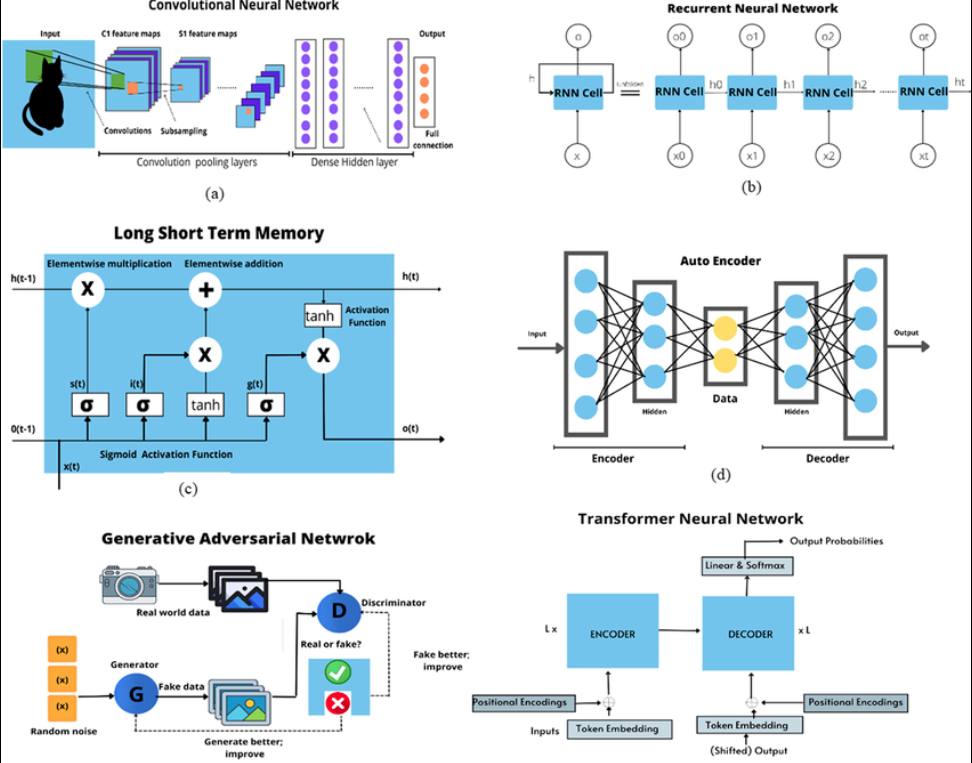
\includegraphics[width=0.8\textwidth]{comparison.png}
\caption{Schematic comparison of CNN, RNN, and ViT architectures (taken from \citealp{MalhotraSingh2025}).}

\label{fig:arch_comparison}
\end{figure}
\newpage
\section{Fundamentals}
Before comparing modern architectures, it is essential to understand the core
ideas that define deep learning models. This section reviews key concepts such
as hierarchical representation learning, spatial and temporal feature
extraction, and global attention mechanisms. It also outlines the fundamental
characteristics of CNNs, RNNs, Vision Transformers, and hybrid systems, setting
the stage for the comparative analysis that follows.
\subsection{Foundational Concepts of Deep Learning}
At its core, deep learning involves the use of neural networks with many layers to automatically extract hierarchical representations from raw data. These networks are designed to learn from large amounts of data by adjusting internal parameters based on backpropagation of errors. The success of deep learning architectures, especially CNNs, RNNs, and ViTs, can be attributed to their ability to capture various levels of abstraction in data, whether spatial, temporal, or global.

\subsection{Convolutional Neural Networks (CNNs)}
CNNs have become the cornerstone of computer vision tasks due to their ability to efficiently capture spatial patterns in images. The architecture consists of convolutional layers, pooling layers, and fully connected layers. CNNs are known for their inductive bias toward locality and translation invariance.

\subsection{Recurrent Neural Networks (RNNs)}
RNNs handle sequential data, maintaining a hidden state that captures previous time steps. Variants like LSTM and GRU improve memory retention across long sequences.

\subsection{Vision Transformers (ViTs)}
ViTs use self-attention to model global relationships in images, dividing images into patches treated as tokens.

\subsection{Hybrid Architectures: Combining CNNs and ViTs}
Hybrid models use CNNs for local feature extraction and transformers for global context. They are effective in domains like medical imaging and human action recognition.

\newpage
\subsection{Comparison}
To highlight the differences between these architectures, Table~\ref{tab:architecture_comparison}
summarizes their strengths, weaknesses, and typical applications. This
comparison provides a high-level view of how CNNs, RNNs, ViTs, and hybrid
models complement each other and where each model family performs best.
\begin{table}[htbp]
\centering
\renewcommand{\arraystretch}{1.3} 
\setlength{\tabcolsep}{10pt} 
\begin{tabular}{|l|l|l|l|}
\hline
\textbf{Architecture} & \textbf{Strengths} & \textbf{Weaknesses} & \textbf{Applications} \\
\hline
CNN & Local features & Poor global context & Image classification \\
RNN & Temporal modeling & Vanishing gradients & NLP, time-series \\
ViT & Global attention & Data-intensive & Large-scale images \\
Hybrid & Local + global & Complex & Medical imaging, video \\
\hline
\end{tabular}
\caption{Comparison of Deep Learning Architectures}
\label{tab:architecture_comparison}
\end{table}

\subsection{Challenges and Research Gaps}
Despite substantial progress, these architectures continue to face practical
and theoretical challenges. Issues such as data efficiency, computational
requirements, optimization stability, and model interpretability remain
active areas of research. This subsection outlines several major gaps that
affect current models and motivate future developments.

\section{Conclusion}
The rapid evolution of neural network architectures has led to significant
advances in performance across vision, language, and multimodal tasks. Yet,
each model family—CNNs, RNNs, ViTs, and hybrid systems—has its own strengths
and unresolved limitations. This conclusion summarizes the key insights
discussed throughout the paper and reflects on opportunities for future
research and architectural innovation.

\newpage

\bibliography{references}

\section*{Cited Notes}

CNNs are highly effective in small-data environments \citep{alzubaidi2021review}. \\

Hybrid models have been explored for spatio-temporal tasks \citep{alomar2024har}. \\

ViTs require large-scale pretraining for optimal performance \citep{khan2023vision}. \\

Medical imaging studies have compared CNNs and ViTs in detail \citep{khan2024medical}. \\

As shown in Figure~\ref{fig:arch_comparison} \citep{MalhotraSingh2025}, the architectures differ in structure and information flow.


\end{document}
